\documentclass[12pt]{exam}

\usepackage{amsmath}
\usepackage{amssymb}
\usepackage{circuitikz}
\usepackage{pgfplots}
\pgfplotsset{compat=1.18}
\usepackage[lmargin=71pt, tmargin=1.2in]{geometry}  %For centering solution box
\thispagestyle{empty}
\begin{document}

\nopointsinmargin
\pointformat{}

\begingroup
\centering
\LARGE PHY 240: Basic Electronics\\
\LARGE Homework Problem H9\\[0.5em]
\large \today\\
\large Aiden Rivera\par
\endgroup

\rule{\textwidth}{0.4pt}

\printanswers
\begin{center}
\begin{circuitikz}[american voltages]
    \node (a) at (4,2) [label=right:a] {};
    \node (b) at (4,0) [label=right:b] {};

    \draw
    (a) to[short, o-] (2,2)
    to[short, nos, mirror, invert] (0,2)
    to[battery1, l_=10V] (0,0)
    to[R, l_=$R$] (2,0)
    to[short, -o] (b)
    (2,2) to[C, l=$1 \, \mu F$] (2,0)
    ;
\end{circuitikz}
\end{center}
\begin{questions}
\question \textbf{Charge Bucket.}\\
\begin{parts}
\part
Consider the circuit above, in which the capacitor is initially uncharged.
In this configuration, and with the output taken between terminals a and b,
would you consider this a “high-pass circuit” or a “low-pass circuit”?

\part
Suppose that we choose a 2 k$\Omega$ resistor for R. If we close the switch at
time $t = 0$, sketch the voltage between terminals a and b, $V_{ab}$, for the time
interval\\ -1 ms $ \leq t \leq $ 2 ms. Make your sketch quantitative, labeling relevant
voltages and times.

\part
Suppose that we now discharge the capacitor completely, replace the 2 k$\Omega$
resistor that we used for R with a 200 $\Omega$ resistor, and again close the switch
at time t = 0. Sketch the voltage that we now see between terminals a and b,
Vab, for the time interval -1 ms $ \leq t \leq $ 2 ms. Make your sketch quantitative,
labeling relevant voltages and times.

\part
Explain clearly how the generic behavior that you sketched in parts (b)
and (c) justifies the name that you gave in part (a).

\end{parts}
\newpage

\begin{solution}
\begin{parts}

% a) 
\part
This is a high pass filter because the low frequencies get consumed by the high impedance of the capacitor before returning to ground through the resistor.
\newpage 

% b) 
\part
With $R = 2\,\text{k}\Omega$\dots
\begin{center}
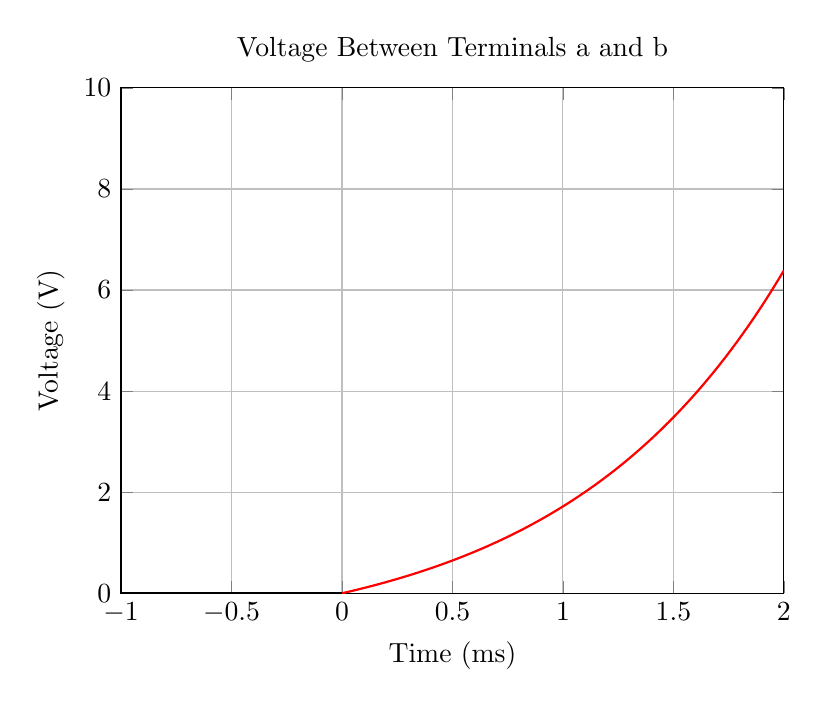
\begin{tikzpicture}
    \begin{axis}[
        width=10cm, height=8cm,
        grid=major,
        xlabel={Time (ms)},
        ylabel={Voltage (V)},
        xmin=-1, xmax=2,
        ymin=0, ymax=10,
        samples=400,
        title={Voltage Between Terminals a and b}
    ]
    % -1:0, switch closed, no voltage
    \addplot[
        domain=-1:0,
        thick,
        color=black
    ]{0};

    % 0:2, switch closed, no voltage
    \addplot[
        domain=0:2,
        thick,
        color=red
    ]{(e^x) -1 };
    \end{axis}
\end{tikzpicture}
\end{center}
\newpage 

% c) 
\part
With $R = 200\,\Omega$\dots
\begin{center}
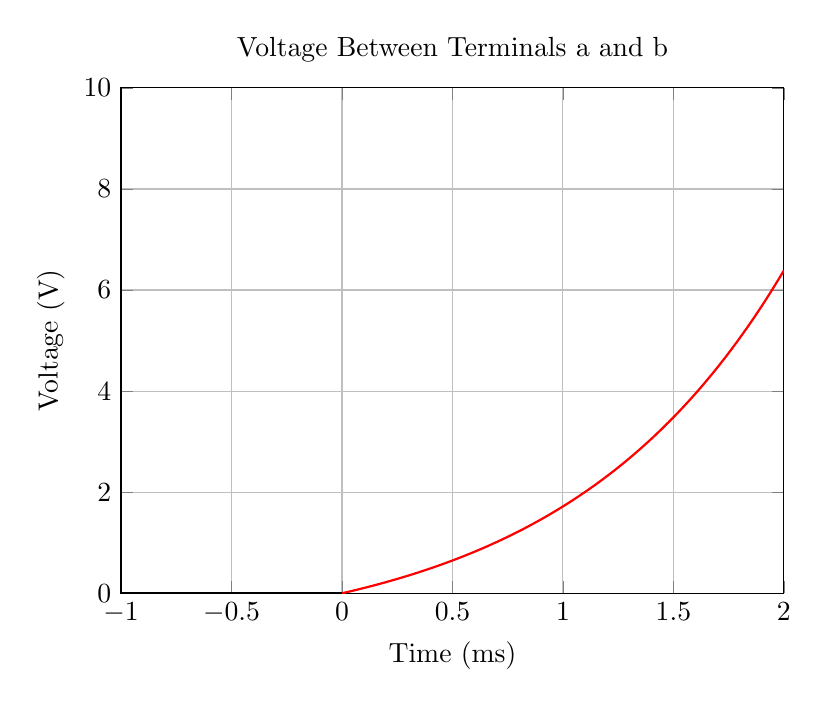
\begin{tikzpicture}
    \begin{axis}[
        width=10cm, height=8cm,
        grid=major,
        xlabel={Time (ms)},
        ylabel={Voltage (V)},
        xmin=-1, xmax=2,
        ymin=0, ymax=10,
        samples=400,
        title={Voltage Between Terminals a and b}
    ]
    % -1:0, switch closed, no voltage
    \addplot[
        domain=-1:0,
        thick,
        color=black
    ]{0};

    % 0:2, switch closed, no voltage
    \addplot[
        domain=0:2,
        thick,
        color=red
    ]{(e^x) -1 };
    \end{axis}
\end{tikzpicture}
\end{center}
\newpage 

% d) 
\part
My brother in christ, what are you talking about
\end{parts}
\end{solution}
\end{questions}
\end{document}
